%
% Copyright (c) 2021 Antonio Coín Castro
%
% This work is licensed under a
% Creative Commons Attribution-ShareAlike 4.0 International License.
%
% You should have received a copy of the license along with this
% work. If not, see <http://creativecommons.org/licenses/by-sa/4.0/>.
%

\RequirePackage{fix-cm}
\documentclass[10pt, english, professionalfonts]{beamer}

\usepackage{pifont}  % xmark, cmark
\newcommand{\cmark}{\ding{51}}%
\newcommand{\xmark}{\ding{55}}%

% OPCIONES DE BEAMER

\definecolor{Maroon}{cmyk}{0, 0.87, 0.88, 0.1}
\definecolor{teal}{rgb}{0.0, 0.45, 0.45}

\usetheme[block=fill, subsectionpage=progressbar, titleformat section=smallcaps]{metropolis}
\setbeamertemplate{frametitle continuation}[roman]
\setbeamertemplate{section in toc}[sections numbered]
%\setbeamertemplate{subsection in toc}[subsections unnumbered]
%\setsansfont[BviejoFont={Fira Sans SemiBold}]{Fira Sans Book}  % Increase font weigth
\widowpenalties 1 10000
\raggedbottom

% COLORES
\setbeamercolor{palette primary}{bg=teal}
\setbeamercolor{progress bar}{use=Maroon, fg=Maroon}

% PAQUETES

\usepackage[utf8]{inputenc}
\usepackage[absolute,overlay]{textpos}
\usepackage[spanish, es-nodecimaldot]{babel}
\usepackage{microtype}
\usepackage{epigraph}
\usepackage{hyperref}
\usepackage{bm}
\usepackage{amssymb, amsmath, amsthm, amsfonts, amscd}
\usepackage{listings}

% FONTS
%\usefonttheme{professionalfonts}
%\usepackage{mathpazo}
%\usepackage{eulervm}

\definecolor{backg}{HTML}{F2F2F2} % Fondo
\definecolor{comments}{HTML}{a8a8a8} % Comentarios
\definecolor{keywords}{HTML}{08388c} % Palabras clave
\definecolor{strings}{HTML}{0489B1}  % Strings

\lstset{
language=scala,
basicstyle=\footnotesize\ttfamily,
breaklines=true,
keywordstyle=\color{keywords},
commentstyle=\color{comments},
stringstyle=\color{strings},
xleftmargin=.5cm,
tabsize=2,
% Acentos, ñ, ¿, ¡ (tex.stackexchange.com/questions/24528)
extendedchars=true
}

% COMANDOS PERSONALIZADOS


\renewcommand{\baselinestretch}{1}
\definecolor{mLightBrown}{HTML}{f97e0b}
\newcommand\maroon[1]{\color{mLightBrown}#1\color{mDarkTeal}}
\let\lmin\wedge
\let\lmax\vee
\newtheorem{prop}{Proposición}
\newtheorem{teorema}{Teorema}
\newtheorem{defi}{Definición}
\newcommand\ddfrac[2]{\frac{\displaystyle #1}{\displaystyle #2}}  % Fracción grande

\renewcommand{\epsilon}{\varepsilon}

\newcommand{\N}{\mathbb{N}}
\newcommand{\R}{\mathbb{R}}
\newcommand{\E}{\mathbb{E}}
\newcommand{\Hcal}{\ensuremath\mathcal{H}}

%% Scalar product
\newcommand\dotprod[2]{\left\langle #1, #2 \right\rangle}

% PLOTS

%\usepackage{pgfplots}
%\DeclareUnicodeCharacter{2212}{−}
%\usepgfplotslibrary{groupplots,dateplot}
%\usetikzlibrary{patterns,shapes.arrows}
%\pgfplotsset{compat=newest}

% TÍTULO

\title{Bayesian methods in RKHS models for functional regression}
\providecommand{\subtitle}[1]{}
\subtitle{Theoretical framework and experiments}
\date{SEIO Congress Granada\\ 8th May 2022\\}
\author{José R. Berrendero \\ Antonio Coín  \\ Antonio Cuevas\\}
\institute{Universidad Autónoma de Madrid \\ \textit{Departamento de Matemáticas}}

\titlegraphic{
  \begin{textblock*}{2cm}(9.8cm, 6.7cm)
    
\includegraphics[width=2cm]{img/logo-uam}
  \end{textblock*}
}
% DOCUMENTO

\begin{document}
\maketitle

\begin{frame}{Table of contents}
  \tableofcontents
\end{frame}

\section{Introduction}

\begin{frame}{FDA: linear regression}
  \textbf{First problem}: \maroon{Linear } regression with functional data.
  \vspace{1em}

\begin{figure}
    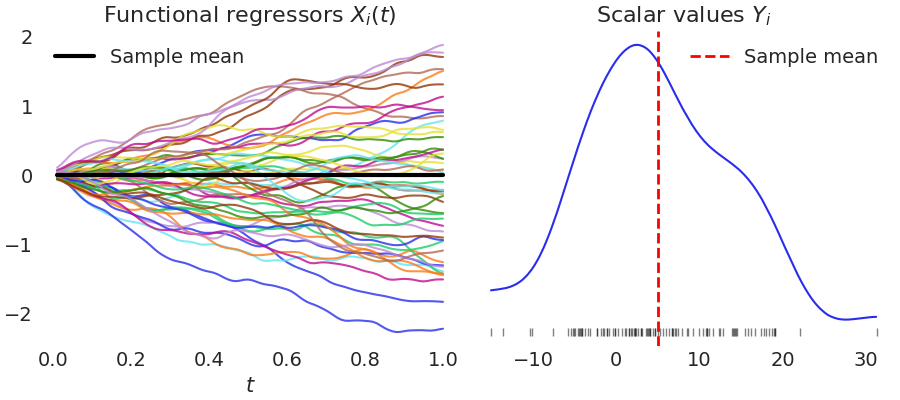
\includegraphics[width=\textwidth]{img/data_lin}
    \caption{Linear regression data set simulated from a fractional brownian motion.}
  \end{figure}
  \vspace{-1em}
\end{frame}
\begin{frame}{FDA: logistic regression}
  \textbf{Second problem}: \maroon{Logistic } regression with functional data.
\vspace{1em}

\begin{figure}
    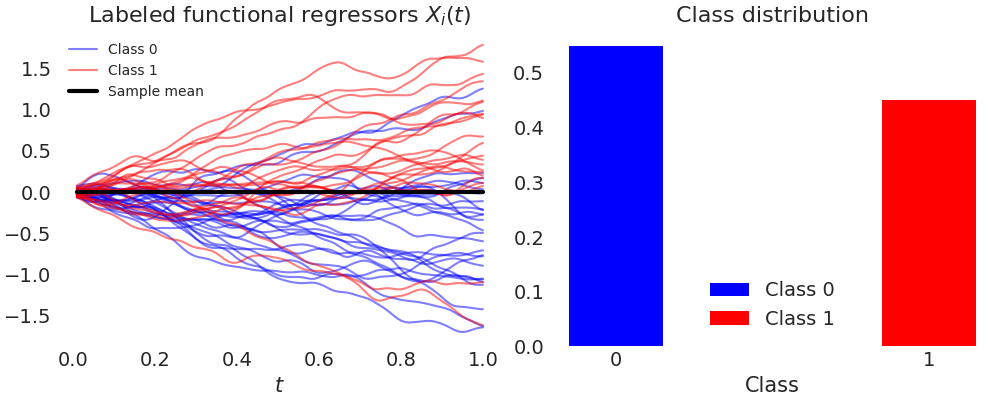
\includegraphics[width=\textwidth]{img/data_log}
    \caption{Logistic regression data set simulated from a fractional brownian motion.}
  \end{figure}
  \vspace{-1em}
\end{frame}

\begin{frame}{Usual models}
  \(\bullet\) \(Y\) real variable (continuous or dichotomous).

  \(\bullet\) \(X(t)\) second order stochastic process with trajectories in \(L^2[0, 1]\).

  \(\bullet\) \(\beta \in L^2[0,1]\) \maroon{functional parameter}.

  \vspace{1em}

\begin{block}{Linear \(\bm{L^2}\)-model}
  \[
    Y = \alpha_0 + \maroon{\langle X, \beta \rangle_2} + \varepsilon = \alpha_0 + \int_0^1 X(t)\beta(t)\, dt + \varepsilon.
  \]
\end{block}
\begin{block}{Logistic \(\bm{L^2}\)-model}
    \[
    \mathbb P (Y=1\mid X) = \frac{1}{\exp\{-\alpha_0 - \maroon{\langle X, \beta\rangle_2}\}} = \frac{1}{\exp\{-\alpha_0 - \int_0^1 X(t)\beta(t)\, dt\}}.
  \]
\end{block}
  \(\alpha_0\in\mathbb R\), \ \(\varepsilon \sim \mathcal N(0, \sigma^2), \ \mathbb E[\varepsilon]=0, \ X \bot \varepsilon\).
\end{frame}


\begin{frame}{Some shortcomings of the \(\bm{L^2}\)-models}
  \begin{itemize}
    \item \(L^2[0, 1]\) is a extremely wide space, which also contains very ill-behaved functions.
    \item The usual least-squares theory cannot be applied directly; some regularization or dimensionality reduction techniques are required.
    \item They do not include simple models based on linear combinations of the marginal of the process as particular cases, such as
    \[
      Y = \alpha_0 + \sum_{j=1}^p \beta_j X(t_j) + \varepsilon.
    \]
    \item In the logistic case, the maximum likelihood estimator does not exist with probability one under fairly general conditions.
  \end{itemize}
\end{frame}

\section{A RKHS model for functional regression}


\begin{frame}{Alternative model: RKHS}

We will exploit the theory of \textit{reproducing kernel Hilbert spaces} (RKHS's).

\vspace{1em}
\begin{alertblock}{Proposal}
  Change the habitat of the functional parameter \(\beta(\cdot)\).
\end{alertblock}

\vspace{1em}
  Instead of assuming \(\beta \in L^2[0, 1]\), we consider \maroon{\(\beta \in \mathcal H(K)\)}, the RKHS associated with the covariance function \(K(t, s)=\mathbb E[X(t)X(s)]\) of the centered process \(X\). Moreover, we substitute \(\dotprod{X}{\beta}_2\) for \maroon{\(\dotprod{X}{\beta}_K\)}.
\end{frame}


\begin{frame}{RKHS essentials}
  \begin{definition}
    Let \(K\) be continuous, and define the preliminary space
    \[
    \Hcal_0(K) = \left\{ f \in L^2[0,1]: \ f(\cdot) = \sum_{i=1}^p a_i K(t_i, \cdot),  p \in \N,  a_i \in \R,  t_i \in [0, 1] \right\},
    \]
    which is endowed with the scalar product \(\dotprod{f}{g}_K = \sum_{i, j} a_i b_j K(t_i, s_j)\), for \(f(\cdot)=\sum_i a_i K(t_i, \cdot) \) and \(g(\cdot)=\sum_j b_j K(s_j, \cdot)\). Then, \(\Hcal(K)\) is the completion of \(\Hcal_0(K)\) under this scalar product.
  \end{definition}

  \vspace{1em}

  Note that \(\Hcal(K)\subset L^2[0, 1]\), but the elements of \(\Hcal(K)\) are simpler and more manageable in general. Plus, the latter is a space of \maroon{functions}, and not of equivalence classes.
\end{frame}


\begin{frame}{Un repaso muy breve de los RKHS's (cont.)}
Se pueden dar otras definiciones equivalentes de \(\Hcal(K)\), basadas en el \textit{operador de covarianzas}
\[
\mathcal Kf(\cdot) = \int_0^1 K(s, \cdot)f(s)\, ds, \quad f\in L^2[0, 1].
\]

\begin{definition}
\begin{enumerate}
  \item  \(\Hcal(K) = \mathcal K^{1/2}(L^2[0, 1])\), con \(\dotprod{f}{g}_K = \dotprod{\mathcal K^{-1/2}(f)}{\mathcal K^{-1/2}(g)}_2\).
  \item \(\Hcal(K) = \{f \in L^2[0, 1]: \ \sum_j \lambda_j^{-1}\dotprod{f}{\phi_j}^2 < \infty \}\), con \(\dotprod{f}{g}_K = \sum_j \lambda_j^{-1}\dotprod{f}{\phi_j}\dotprod{g}{\phi_j}_2\). En este caso, \(\lambda_j\) y \(\phi_j\) son los autovalores y autofunciones de \(\mathcal K\).
\end{enumerate}
\end{definition}

La segunda de estas definiciones enfatiza el hecho de que las funciones de \(\Hcal(K)\) son ``simples'', en el sentido de que sus componentes en una base ortonormal tienden a \(0\) rápidamente.

\end{frame}

\begin{frame}{A small subtlety}

  Generally speaking, the concrete realizations \(x=X(\omega)\) \maroon{do not belong to \(\Hcal(K)\) with probability \(1\)}, so the expression \(\dotprod{x}{\beta}_K\) lacks meaning. However, we can make use of the relationship between \(\Hcal(K)\) and \(\mathcal L(X)\), the linear span of the process \(X\) within \(L^2(\Omega)\).


  \vspace{1em}
  \begin{block}{Loève's isometry}
    It is the completion of the correspondence
    \[
\sum_{j=1}^p a_j X(t_j) \longleftrightarrow \sum_{j=1}^p a_j K(t_j, \cdot).
    \]
    Formally, \(\Psi^{-1}_X(U)(t) := \E[U X(t)]\) for \(U \in \mathcal L(X)\).
  \end{block}
  With a slight abuse of notation, we will write \maroon{\(\dotprod{x}{\beta}_k \equiv \Psi_x(\beta)\)}. This correspondence will allow us to still call our models ``linear''.
\end{frame}


\begin{frame}{A new functional parameter...}
  \begin{itemize}
    \item The initial idea was to suppose \(\beta \in \Hcal(K)\).
    \item To further simplify the model, we will assume \(\beta \in \Hcal_0(K)\), which is dense in \(\Hcal(K)\) by construction. That is,
    \[
      \beta(\cdot) = \sum_{j=1}^p \beta_j K(t_j, \cdot).
    \]
    \item When evaluating \(\dotprod{x}{\beta}_K\) for a trajectory \(x=X(\omega)\), we resort to Loeve's isometry:
    \[
      \dotprod{x}{\beta}_K = \Psi_x(\beta) = \sum_{j=1}^p \beta_j X(t_j).
    \]
  \end{itemize}

\end{frame}


\begin{frame}{...and two new models}
  Given a data set \(\mathcal D_n = \{(X_i, Y_i): i=1,\dots, n\}\) composed of i.i.d. samples of \((X, Y)\), we consider:

  \vspace{1em}

  \begin{block}{Linear RKHS model}
  \[
    Y_i = \alpha_0 + \maroon{\langle X_i, \beta \rangle_K} + \varepsilon = \alpha_0 + \sum_{j=1}^p \beta_j X_i(t_j) + \varepsilon.
  \]
\end{block}
\begin{block}{Logistic RKHS model}
    \[
    \mathbb P (Y_i=1\mid X_i) = \frac{1}{\exp\{-\alpha_0 - \maroon{\langle X_i, \beta\rangle_K}\}} = \frac{1}{\exp\{-\alpha_0 - \sum_{j=1}^p \beta_j X_i(t_j)\}}.
  \]
\end{block}
\end{frame}

\begin{frame}{Benefits of the RKHS models}
  \begin{itemize}
    \item MLE existe..
    \item El modelo es verdadero en algunos casos...
  \end{itemize}
\end{frame}

\section{A bayesian approach}

\begin{frame}{Parameter estimation}

  We have a parameter vector \(\theta = (p, \beta_1,\dots, \beta_p, t_1,\dots, t_p, \alpha_0, \sigma^2)\), on which we impose a prior distribution \(\pi(\theta)\). In practice, we are establishing a prior distribution on the functional space \(\Hcal(K)\) via a density argument.

  \vspace{1em}

  Afterwards we apply \textit{Bayes'}  theorem in the usual way to obtain the posterior distribution of the parameters given the data.

  \begin{block}{Bayes's theorem}
      \[
      \pi(\theta \mid \mathcal D_n) \propto \left( \prod_{i=1}^n \pi(Y_i\mid X_i, \theta) \right)\pi(\theta).
      \]
  \end{block}
  \vspace{1em}

  Finally, we obtain samples of the approximate posterior distribution using an algorithm of the family of \textit{Markov chain Monte Carlo} (MCMC) methods.

\end{frame}

\begin{frame}{Prior distributions}
  Same prior scenario for both linear and logistic models.
  \begin{block}{Prior de los parámetros}
    \vspace{-1em}
  \begin{align*}
    p &\sim \text{Categorical}(p_{\text{max}}),\\
  \pi(\alpha_0, \sigma^2)              & \propto 1/\sigma^2,                                                     \\
  \tau                     & \sim \mathcal U([0, 1]^p),                                              \\
  \beta\mid \tau, \sigma^2 & \sim \mathcal N\big(b_0, g\sigma^2{\underbrace{\left[\mathcal X_\tau' \mathcal X_\tau + \eta I\right]}_{G_\tau}}^{-1}\big),
\end{align*}
where \(I\) is the identity matrix, \(\mathcal X_\tau = (X_i(t_j))_{i,j}\), and \(b_0\in \R^p, \ g \in \R\) and \(\eta \in \R^+\) are hyperparameters.
\end{block}

\metroset{block=transparent}

\begin{alertblock}{Hyperparameter selection}
  \vspace{0.1em}
  For \(b_0\) we use a computational approximation of the MLE; the rest of hyperparameters are set via \textit{cross-validation}.
\end{alertblock}
\metroset{block=fill}
\end{frame}

\begin{frame}{Posterior distributions}
  \begin{block}{Linear log-posterior}
    \vspace{-1em}
    \begin{align*}
  \log \pi(\theta\mid \mathcal D_n) &\propto \frac{1}{2}\log |G_\tau| - (p+n)\log \sigma\\
  &-\frac{1}{2\sigma^2} \left(\|\boldsymbol{Y}-\alpha_0\boldsymbol{1} - \mathcal X_\tau\beta\|^2 + \frac{1}{g}(\beta - b_0)'G_\tau(\beta - b_0) \right),
\end{align*}
where \(\bm Y=(Y_1,\dots,Y_n)'\) y \(\bm{1}\) is an \(n\)-dimensional vector of ones.
  \end{block}

\vspace{1em}
  \begin{block}{Logistic log-posterior}
      \vspace{-1em}
    \begin{align*}
  \log \pi(\theta \mid \mathcal D_n) \propto {} & \sum_{i=1}^n \left[ \left(\alpha_0 + \Psi_{X_i}(\alpha)\right)Y_i - \log\left(1 + \exp\left\{\alpha_0 + \Psi_{X_i}(\alpha)\right\}\right)\right]\\
  \quad &+ \frac{1}{2}\log |G_\tau| - p\log \sigma -\frac{1}{2g\sigma^2} (b - b_0)'G_\tau(b - b_0).
\end{align*}
Remember that \(\Psi_{X_i}(\alpha) = \sum_j \beta_j X_i(t_j)\).
  \end{block}
\end{frame}

\begin{frame}{Posterior approximation}
  We use the Python library \maroon{emcee}, which implements an MCMC algorithm consisting on multiple chains that interact with each other to advance on each step (\textit{Affine-invariant ensemble sampler}).

  \vspace{1em}

  \begin{figure}
    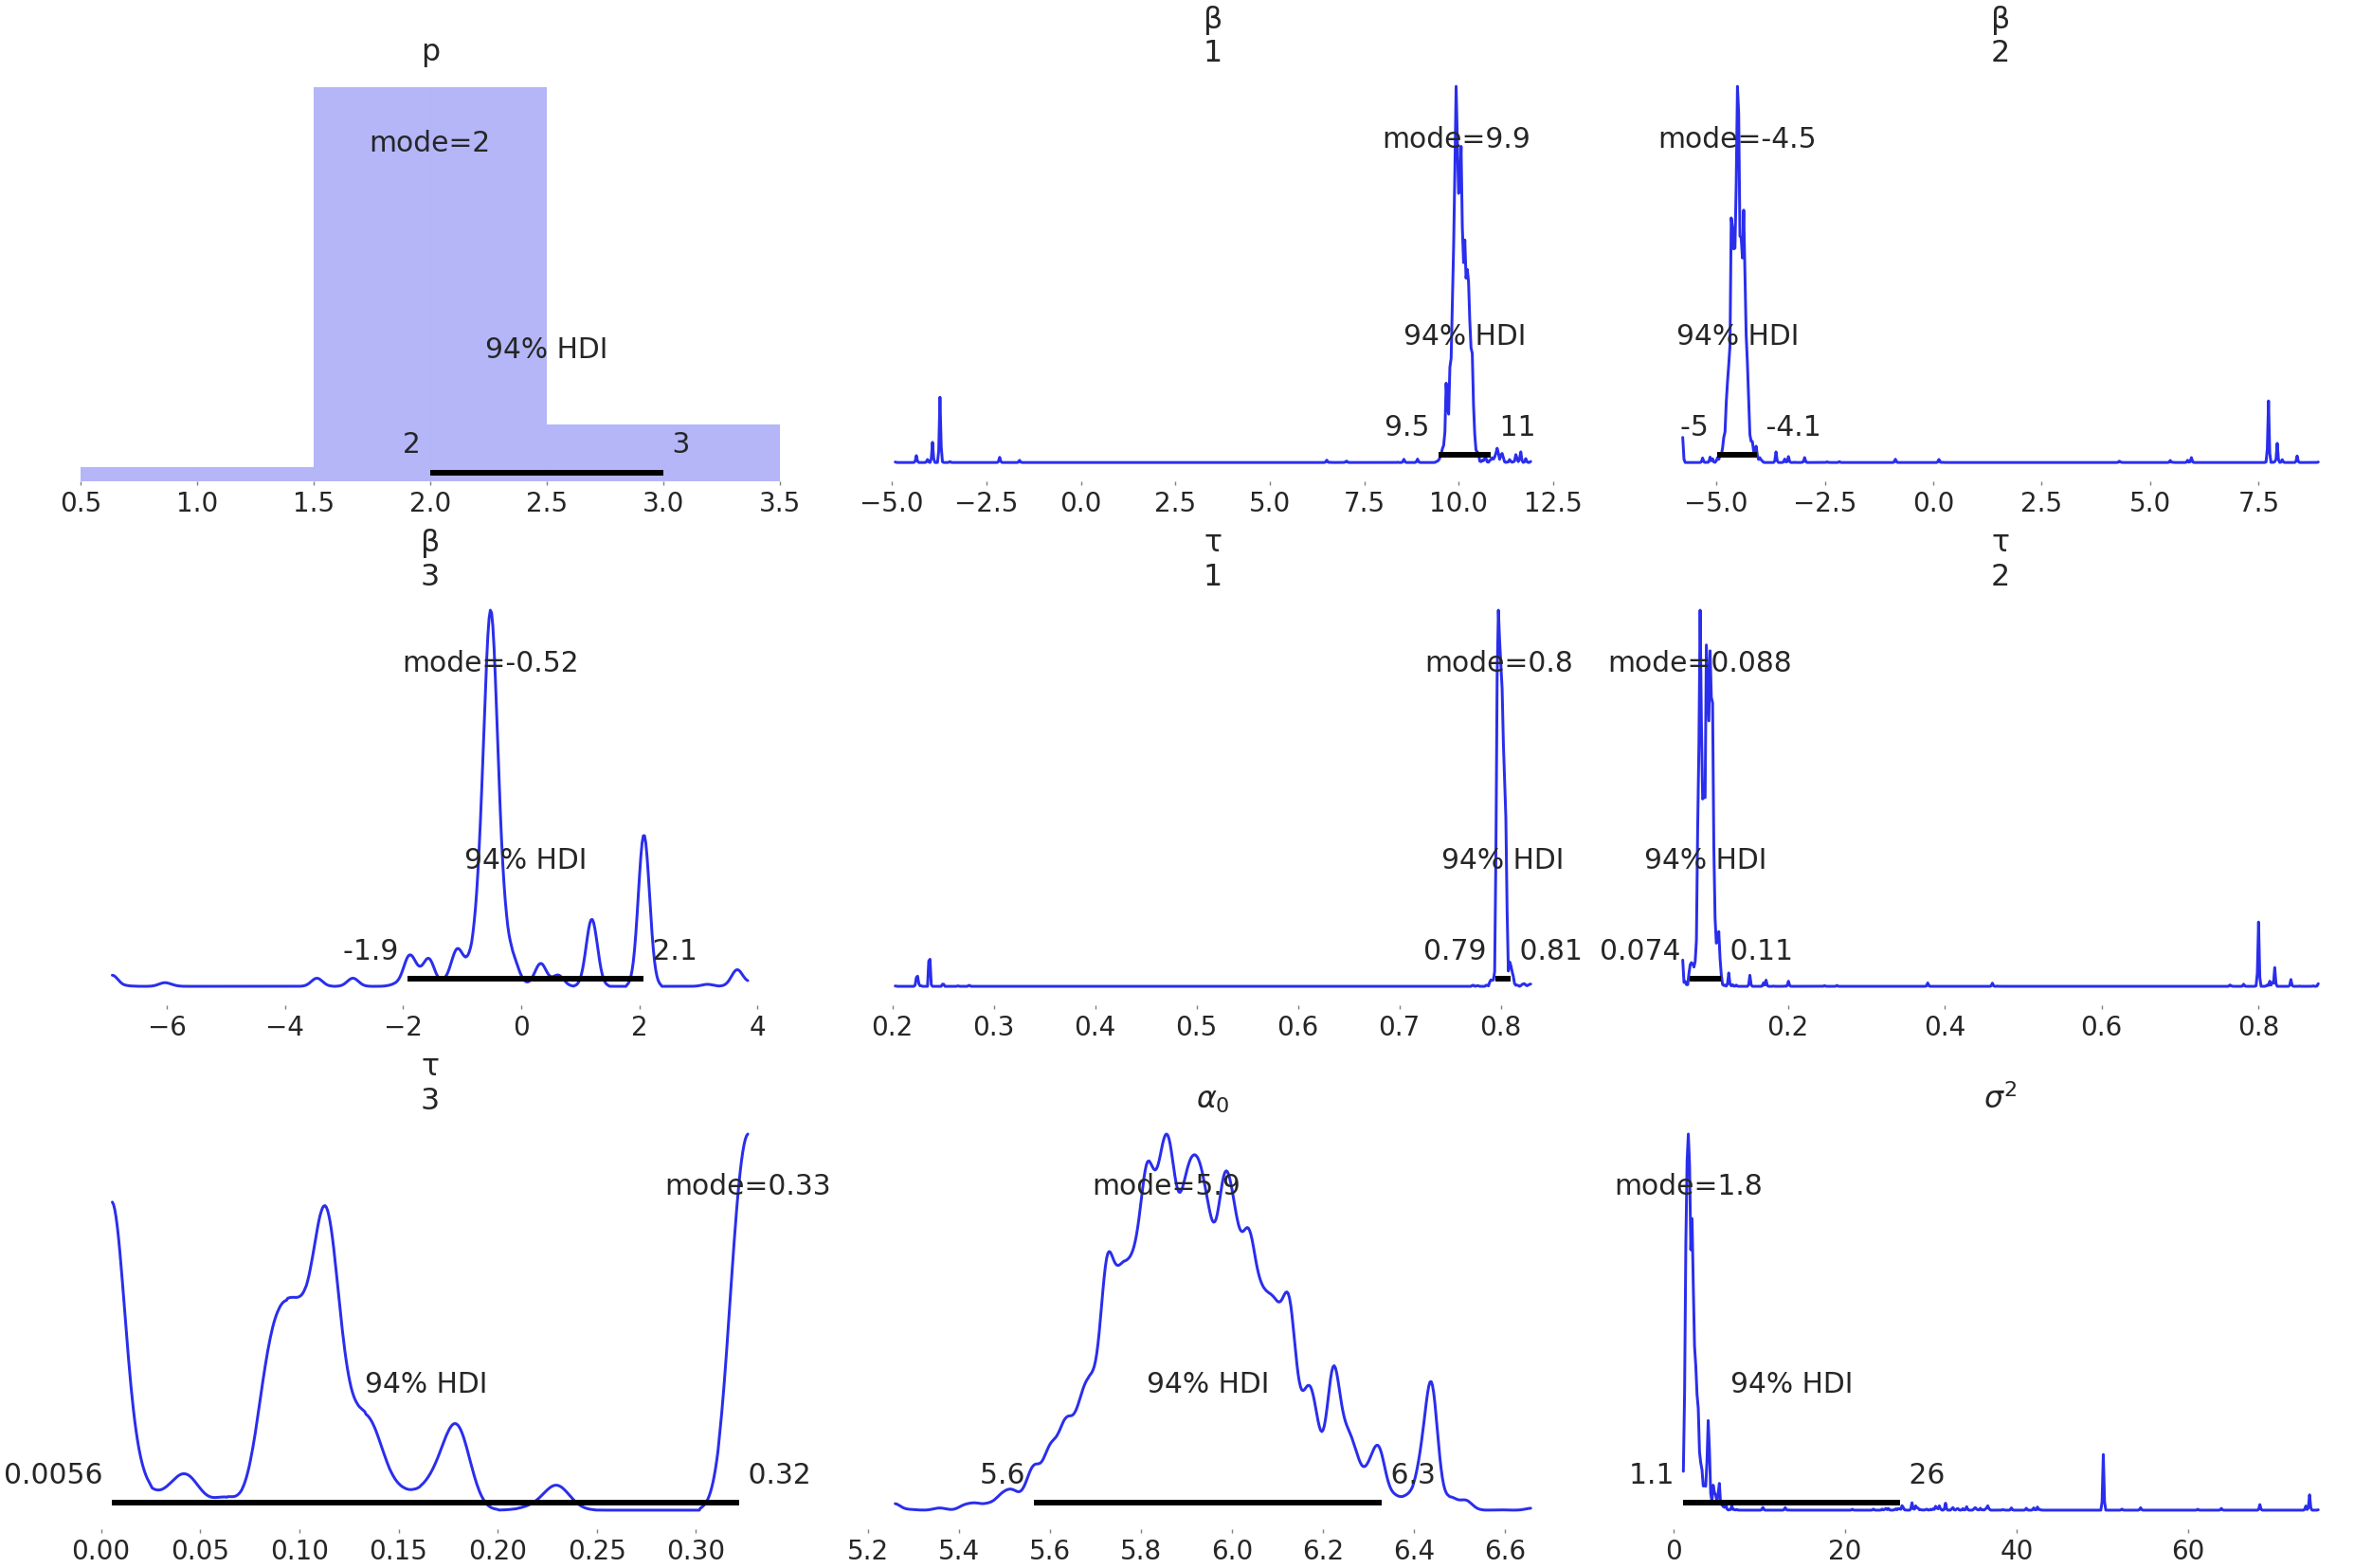
\includegraphics[width=.7\textwidth]{img/posterior}
    \caption{Estimated posterior distribution \(\theta|\mathcal D_n\).}
  \end{figure}
\end{frame}

\begin{frame}{Predictions}
  \textbf{Summarize-then-predict}. A summary of the posterior distribution \(\theta| \mathcal D_n\) is obtained via a point-estimate statistic (mean, median, mode), and then predictions are made according to the assumed model, e.g.:
  \[
  \hat Y_i =\hat \alpha_0 + \sum_{j=1}^p \hat \beta_j X_i(\hat \tau_j), \quad i=1,\dots, n.
  \]

  \textbf{Predict-then-summarize}. For each MCMC iteration we get a sample \(\theta^{(m)*}\) of the approximate posterior. We first construct predictions on each step following our model, i.e.:
  \[
    Y_i^{(m)*} \equiv Y_i \mid X_i, \theta^{(m)*}, \quad m=1,\dots,M, \quad i=1,\dots, n.
  \]

  Then, the mean of all such intermediate predictions (\textit{posterior predictive distribution}) is used as a proxy for the response variable:
  \[
    \hat Y_i = \frac{1}{M}\sum_{m=1}^M Y_i^{(m)*}, \quad i=1,\dots, n.
  \]

\end{frame}

\begin{frame}{Predictions (cont.)}
    \textbf{Variable selection}. We select \(p\) variables using only a point estimator of \(\tau=(t_1,\dots, t_p)|\mathcal D_n\) (so-called \textit{impact points}), and then we can apply any multiple regression algorithm to the reduced data set.
    \vspace{1em}

    \begin{figure}
      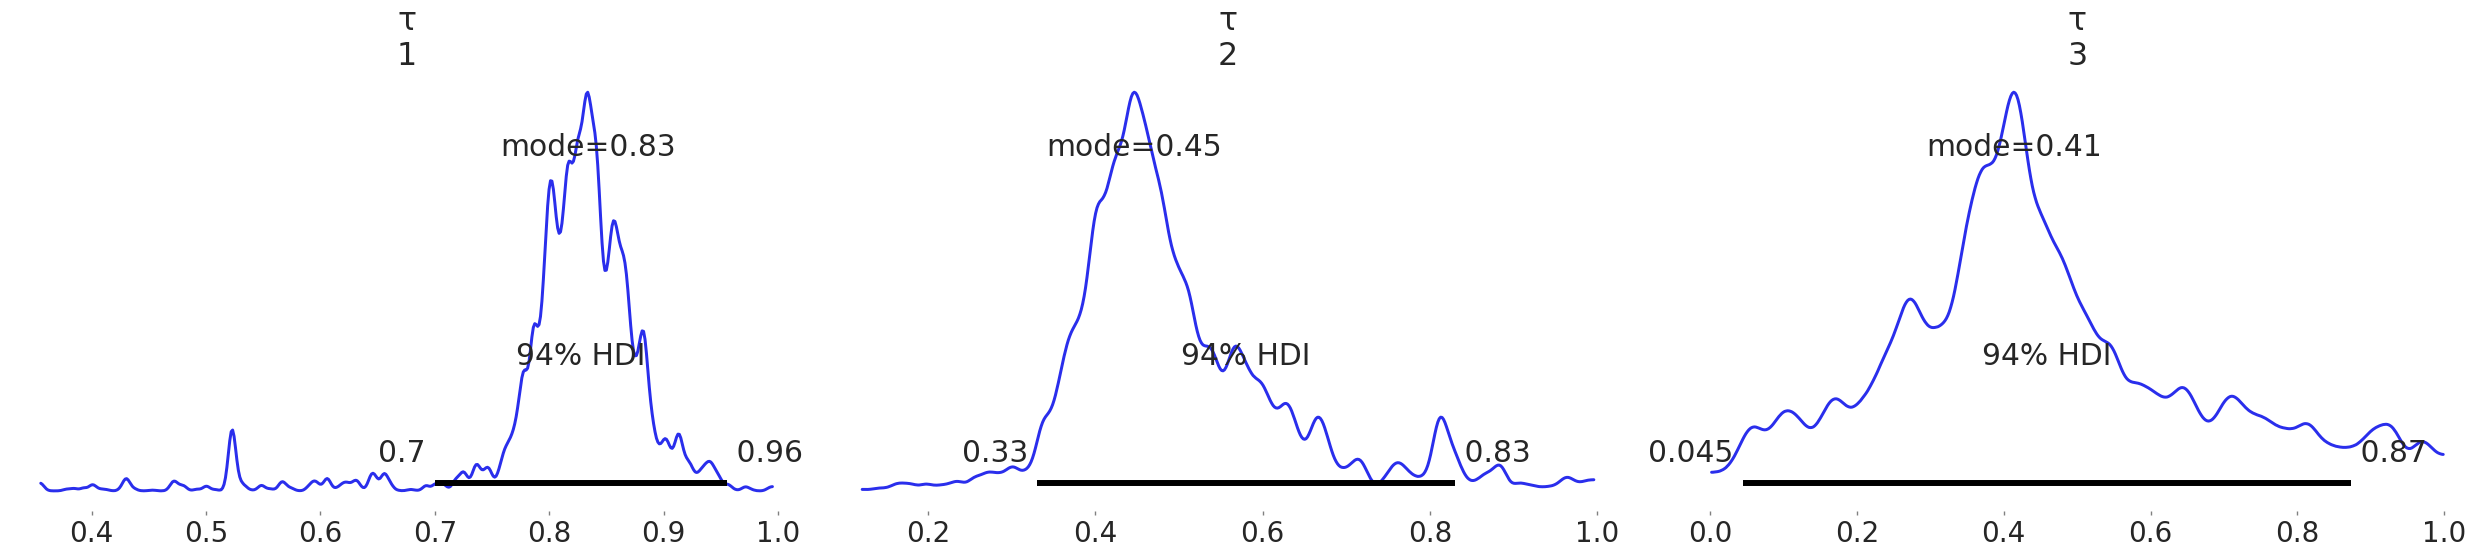
\includegraphics[width=\textwidth]{img/tau_posterior}
      \caption{Approximate posterior distribution for the impact points.}
    \end{figure}

    At any rate, all the above predictors can be obtained after a single run of the MCMC algorithm.
\end{frame}

\subsection{Validación de modelos}

\begin{frame}{Model checking}
  \begin{itemize}
    \item Análisis de la traza de las cadenas y de la distribución a posteriori de los parámetros. Se obtienen directamente \maroon{intervalos creíbles } para los parámetros.
    \item \textit{Bayesian p-values}: \(\tilde p=P(T(Y^*)\leq T(Y)\mid Y)\) para ciertas elecciones de \(T\): mínimo, máximo, mediana, media, etc. Se calcula contando la proporción de muestras aproximadas que cumplen la desigualdad, y se espera que esté en torno a \(0.5\).
    \item Análisis descriptivo y visual de la distribución a posteriori predictiva, tanto con los datos de entrenamiento como con nuevos datos de validación.
  \end{itemize}

\end{frame}

\begin{frame}{Model checking (cont.)}
  \begin{figure}
    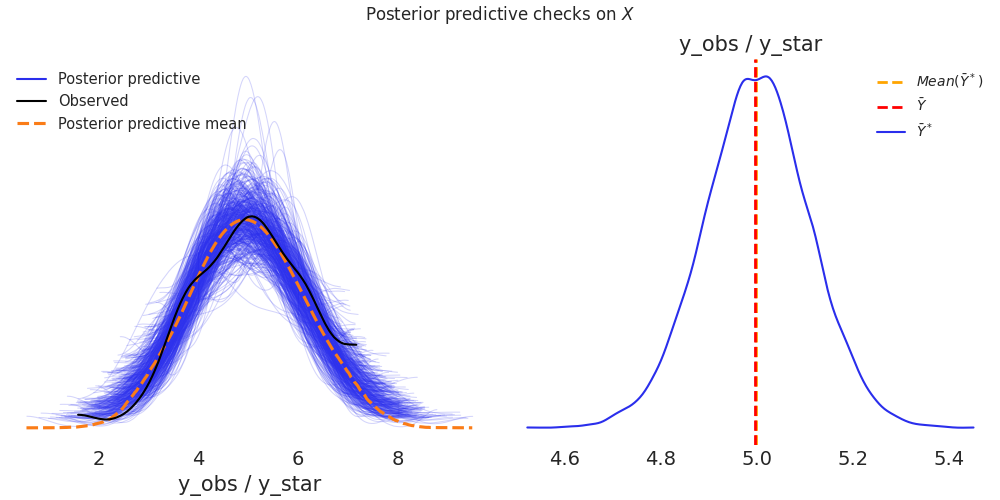
\includegraphics[width=\textwidth]{img/ppc_linear}
    \caption{\textit{Posterior predictive checks} para regresión lineal.}
  \end{figure}
\end{frame}

\begin{frame}{Model checking (cont.)}
  \begin{figure}
    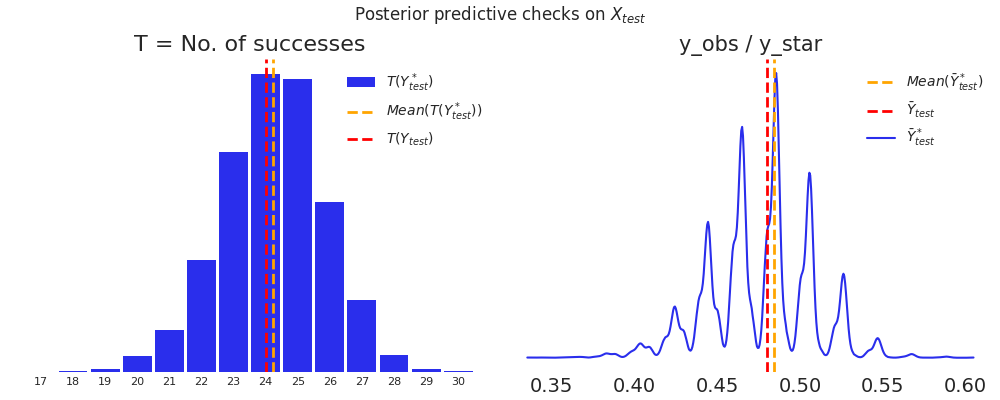
\includegraphics[width=\textwidth]{img/ppc_logistic1}
    
\includegraphics[width=\textwidth]{img/ppc_logistic2}
    \caption{\textit{Posterior predictive checks} para regresión logística.}
  \end{figure}
\end{frame}

\section{Experimentos}

\begin{frame}{Metodología}
  \begin{itemize}
    \item Por motivos prácticos, consideramos la posibilidad de fijar el valor de \(p\) de antemano, considerándolo como un hiperparámetro más del modelo (equivalente a una distribución a priori degenerada).
  \end{itemize}
\end{frame}

\begin{frame}{Datos sintéticos}
  Se consideran 150 ejemplos de \(X \sim GP(0, K(s, t))\) y tres posibles variantes de \(K\): movimiento browniano fraccional (\(H=0.8\)), Ornstein-Uhlenbeck y kernel RBF.

  Se genera la respuesta \(Y\) acorde a dos modelos, RKHS y \(L^2\). Concretamente, se elige
  \[
    Y_i \sim \mathcal N\big(5 -5X_i(0.1) + 10X_i(0.8), \ 0.5\big)
  \]
  ó
  \[
    Y_i \sim \mathcal N\left(5 + \int_0^1 \log(1+4t)X_i(t)\, dt, \ 0.5\right).
  \]

Consideramos una malla regular de \(N=100\) puntos en \([0, 1]\), y un reparto de 100 ejemplos para entrenamiento y 50 para evaluación.
\end{frame}

\begin{frame}{Datos reales}
  Se consideran dos conjuntos de datos reales.
  \begin{itemize}
    \item \textbf{Tecator:} Contiene 215 ejemplos de mediciones de \textit{absorbancia} en muestras de carne para intentar predecir su contenido en grasa.
    \item \textbf{Aemet}: Contiene 73 ejemplos de curvas de temperatura, a partir de las cuales se intenta predecir la precipitación total.
  \end{itemize}

  En ambos casos hacemos una división \(80\%-20\%\) para entrenamiento y \textit{test}.
\end{frame}

\begin{frame}{Preprocesado de los datos}
  \begin{itemize}
    \item Se centran los regresores para que tengan media \(0\). Opcionalmente, se pueden estandarizar en cada punto de la malla.
    \item Se permite \textbf{sustituir los datos \(\boldsymbol{X_i}\) por su desarrollo en una base} de Fourier, con un número determinado de coeficientes. De esta forma realizamos un suavizado de las curvas.
  \end{itemize}
\end{frame}

\begin{frame}{Algoritmos de comparación}
  \textbf{Regresión lineal multivariante:} Regresión Lineal estándar, Lasso (\(L^1\)), Ridge (\(L^2\)).

  \textbf{Regresión no lineal multivariante}: SVM con kernel RBF.

  \textbf{Regresión lineal funcional}: Modelo \(L^2\), KNN Funcional.

  \textbf{Reducción de dimensión:} PCA Funcional (proyección sobre coeficientes).

  \textbf{Selección de variables:} Aleatoria.

  \vspace{1em}

  Se entrenan todos ellos sobre el conjunto de entrenamiento, haciendo \textit{5-fold cross validation} para escoger los mejores hiperparámetros en cada caso (valor de regularización, número de componentes, ...).
\end{frame}

\begin{frame}{Metodología experimental}
  \begin{itemize}
  \item Para cada conjunto de datos consideramos tres posibles valores de \(p\) y cuatro posibles valores de \(\eta\):
  \begin{itemize}
    \item[--] \(p\in \{2,3,4\}\) para los datos sintéticos y \(p\in \{3, 4, 5\}\) para los datos reales.
      \item[--] \(\eta \in \{0.01, 0.1, 1.0, 10.0\}\).
  \end{itemize}

  \item Para aumentar la estabilidad hacemos 5 repeticiones de cada modelo. Es decir, entrenamos un total de 60 modelos sobre el conjunto de entrenamiento

  \item Con el \textbf{mejor modelo obtenido} se realiza también una selección de variables basada en los valores de \(\tau\) estimados mediante los distintos estimadores puntuales.
\end{itemize}

Además, repetimos este proceso con los datos suavizados en una base de Fourier con 11 elementos (también con los algoritmos de comparación).
\end{frame}

\begin{frame}{Metodología experimental (cont.)}
  Fijamos algunos hiperparámetros:
  \begin{itemize}
    \item Número de cadenas: 64.
    \item Número de pasos: 100 + 1000.
    \item Movimientos: elección aleatoria (ponderada) entre dos de los recomendados, \textit{stretch} y \textit{walk}.
    \item Inicialización: Entorno aleatorio del MLE + muestras de las distribuciones a priori.
    \item Prior de \(\beta\): \(b_0\) se elige como el MLE de \(\beta\), y fijamos \(g=5\) (recomendado en \textit{Grollemund et al. (2019)}).
  \end{itemize}
  \vspace{1em}

  \textit{Nota:} El valor de \(g\) no parece afectar al resultado, por lo que podríamos eliminar este parámetro.
\end{frame}

\begin{frame}{Resultados L2}
  \begin{figure}
    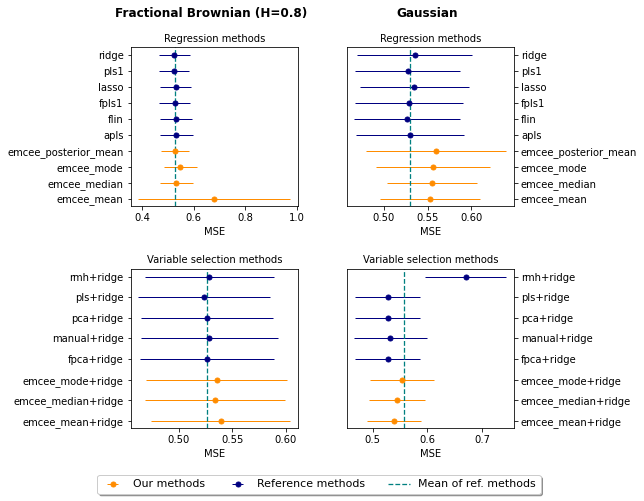
\includegraphics[width=\textwidth]{img/reg_emcee_l2}
    \caption{caption.}
  \end{figure}
\end{frame}

\begin{frame}{Algunas observaciones}
\begin{itemize}
  \item Por cada modelo entrenado obtenemos 4 estimadores y 3 estrategias de selección de variables.
  \item En general, se obtienen mejores resultados con el uso de la base.
  \item El tiempo medio de entrenamiento de cada modelo es de unos 20-30 segundos.
  \item En ocasiones, nuestro algoritmo supera con holgura a todos los algoritmos de comparación. Cuando pierde, suele ser frente a uno o dos de ellos (y por poco), pero sigue superando al resto.
  \item Se puede considerar como algoritmo de comparación el estimador de máxima verosimilitud de los parámetros. En casi todas las pruebas experimentales, el desempeño de nuestro algoritmo supera al del MLE.
\end{itemize}

\end{frame}

\begin{frame}{Dificultades}
  \begin{itemize}


  \item Hay multitud de grados de libertad: estandarización de regresores y/o variable respuesta, elección o no de una base (¿cuál?,) algoritmo de estimación del MLE, número, longitud y movimientos de las cadenas MCMC, elección de distribuciones a priori, elección de \(g, b_0\) y \(\eta\), etc.
  \item El algoritmo MCMC es costoso, y en conjuntos de datos grandes las estrategias de \textit{cross-validation} para seleccionar parámetros pueden no ser viables.
  \item Es necesario un procedimiento para seleccionar el valor de \(p\) (BIC, WAIC, WBIC, \textit{cross-validation}, ...).
  \item Debido a la aleatoriedad del algoritmo, los resultados pueden variar sustancialmente de una ejecución a otra.
  \item La distribución a priori para \(\beta\) depende en gran medida del valor de \(b_0\) escogido. Si su estimación inicial no es buena, el algoritmo no funciona demasiado bien.
\end{itemize}
\end{frame}

\begin{frame}{Dificultades (cont.)}
  \begin{itemize}
    \item Hay un problema de \textit{identificabilidad} de los coeficientes (son intercambiables), que se agudiza especialmente al usar varias cadenas.
    \item En el caso en el que el modelo subyacente es RKHS, es posible que no se recuperen los verdaderos valores de los parámetros debido a interacciones entre los coeficientes (si \(p\) es mayor que el número real de componentes).
    \item El uso de distribuciones a priori impropias implica comprobar que \(\int_{\Theta} \pi(Y\mid \theta)\pi(\theta)\, d\theta < \infty\).
  \end{itemize}
\end{frame}

\begin{frame}{Alternativas}
  \begin{itemize}
    \item Explorar el concepto de \textit{online learning} aplicado a esta situación, por ejemplo usando como priori de nuevos datos la posteriori aprendida. Estudiar la \textbf{consistencia} de la distribución a posteriori.
    \item Utilizar otras herramientas de suavizado en lugar de bases de Fourier.
    \item Sustitutir la distribución a priori de \(\beta\) por otra que requiera menos hiperparámetros.
    \item Sustituir las distribuciones impropias por otras propias.
  \end{itemize}

\end{frame}

\section{Regresión Logística Funcional Bayesiana}

\subsection{Marco teórico}

\begin{frame}{Planteamiento Bayesiano}
\textbf{Modelo}: Cada \(Y_i\) se puede ver como una variable aleatoria de Bernoulli \(\mathcal B(p(x_i))\), con
\[
p_i \equiv p(x_i)=\mathbb P(Y_i=1\mid X_i=x_i) = \frac{1}{1 + \exp\left\{-\alpha_0-\displaystyle\sum_{j=1}^p \beta_jx_i(\tau_j)\right\}}.
\]

\end{frame}

\begin{frame}{Predicciones}

\begin{itemize}
  \item Fijamos un umbral en \(0.5\) para establecer la pertenencia a las clases.
   \item Los estimadores puntuales y la selección de variables son análogos al caso de regresión lineal.
   \item Tenemos ahora dos estimadores basados en la distribución a posteriori (similares a los \textit{ensembles} de clasificadores):
   \begin{itemize}
     \item[--] Basado en el voto mayoritario de las muestras \(Y^*\) generadas.
     \item[--] Basado en la media de las probabilidades \(p_i^*\) generadas (con aplicación posterior del umbral).
   \end{itemize}
  \item Se usa el \textit{accuracy} (precisión) para evaluar los modelos.
\end{itemize}
\end{frame}

\subsection{Experimentos}

\begin{frame}{Datos sintéticos}
Seguimos la misma estrategia de generación de datos antes. Se consideran las mismas tres funciones de covarianza y se genera la respuesta tanto con un modelo RKHS como L2, i.e.:
  \[
    Y_i \sim \mathcal B\left(\frac{1}{1 + \exp\left\{0.5 + 5X_i(0.1) - 10X_i(0.8)\right\}}\right)
  \]
  ó
  \[
    Y_i \sim \mathcal B\left(\frac{1}{1 + \exp\left\{0.5 -\int_0^1 \log(1+4t)X_i(t)\, dt\right\}}\right).
  \]

  \vspace{1em}

  Se introduce un pequeño ruido aleatorio en las etiquetas, y además se intenta que ambas clases estén balanceadas.

\end{frame}

\begin{frame}{Datos reales}
  Se consideran dos conjuntos de datos reales.
  \begin{itemize}
    \item \textbf{Medflies:} Contiene 534 ejemplos de mediciones del número de huevos diario puesto por una serie de moscas, para intentar predecir si viven mucho o poco.
    \item \textbf{Growth}: Contiene 93 ejemplos de curvas de altura en niños y niñas.
  \end{itemize}

  En ambos casos hacemos una división \(80\%-20\%\) para entrenamiento y \textit{test}.
\end{frame}

\begin{frame}{Algoritmos de comparación}
  \textbf{Clasificación lineal multivariante:} Regresión Logística, SVM lineal.

  \textbf{Clasificación no lineal multivariante}: SVM con kernel RBF.

  \textbf{Clasificación funcional}: \textit{Maximum Depth}, \textit{Nearest Centroid} Funcional, KNN Funcional.

  \textbf{Reducción de dimensión:} PCA Funcional (proyección sobre coeficientes).

  \textbf{Selección de variables:} Aleatoria, \textit{Recursive Maxima Hunting}, \textit{RKVS} (Mahalanobis).

  \vspace{1em}

  Mismo preprocesado y metodología experimental que en el caso de regresión lineal, utilizando esta vez 9 coeficientes de Fourier.
\end{frame}

\end{document}
